\documentclass[11pt]{beamer}
\usetheme{Goettingen}
\usepackage[utf8]{inputenc}
\usepackage{amsmath}
\usepackage{amsfonts}
\usepackage{amssymb}
\usepackage{graphicx}
\usepackage{hyperref}
\author{Qimin Yan, Alex Heilman}
\title{Crystal Hypergraph Neural Networks}
\subtitle{A Universal Framework for Material System Machine Learning}
%\setbeamercovered{transparent} 
%\setbeamertemplate{navigation symbols}{} 
%\logo{} 
%\institute{} 
%\date{} 
%\subject{} 

\newenvironment{boxed2}
    {\begin{center}
    \begin{tabular}{|p{0.95\textwidth}|}
    \hline\\
    }
    { 
    \\\\\hline
    \end{tabular} 
    \end{center}
    }


\begin{document}

\begin{frame}
\titlepage
\end{frame}

%\begin{frame}
%\tableofcontents
%\end{frame}

\begin{frame}{Machine Learning on Crystal Systems}
To perform predictive tasks for material systems, such as crystalline structures, we essentially need two things:

\medskip

$\bullet$ A way to represent the material system mathematically

\medskip

$\bullet$ A trainable predictive model or set of functions which takes, as input, the material system's representation (as well as a large set of data)
\end{frame}


\section{Crystal Graphs}
\begin{frame}{Usual Crystal Graph Construction \small(a la CGCNN)}

The usual technique is to represent crystalline systems as graphs (nodes and edges), with atomic features associated with nodes and geometric features associated with edges

\medskip

\begin{center}

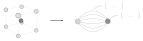
\includegraphics[scale=0.7]{crystalgraph.pdf}

\end{center}
\end{frame}

\begin{frame}{Crystal Graphs cont. I}

$\bullet$ Edges are determined by distance cutoff (4 Ang.) and maximum number of neighbors (12)

\begin{center}
\includegraphics[scale=0.45]{ex_bondcriteria.pdf}
\end{center}
\end{frame}

\begin{frame}{Crystal Graphs cont. II}
Edge attributes then are a Gaussian distance expansion

\begin{center}
\includegraphics[scale=0.33]{bond_feat.pdf}
\end{center}
\end{frame}

\begin{frame}{Message Passing on Graphs}
Now, we need to update these features through some trainable function that acts on graph representations.


\medskip

This is most generally accomplished by a message passing network applied to graph representations.
\begin{gather*}
m_i^{t+1}=\sum_{n_j\in \mathcal{N}(i)} M_t(n_i^{t},e_{ij},n_j^t )\\
\\
n_i^{t+1}=U_t(n_i^t,m_i^{t+1})\\
\end{gather*}
Here, each node $n$ from layer $t$ to $t+1$ is updated according to an update function $U$, which takes as input messages formed from each pair of nodes containing the node to be updated.
\end{frame}

\begin{frame}{Graph Limitations}
Problem: Our underlying representation encodes only distances between atoms!

\begin{center}

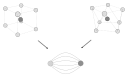
\includegraphics[scale=0.7]{crystalgraph_cntex.pdf}

\end{center}

So, as a rough example, the above two crystalline structures would have the same representations!
\end{frame} 

\section{Crystal Hypergraphs}
\begin{frame}{Solution: Hypergraphs!}
Hypergraphs allow us to have edges containing more than (or less than) two nodes.

\begin{center}
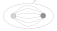
\includegraphics[scale=0.7]{hyperedge_ex.pdf}
\end{center}

This gives us a natural way to encode features with higher order structure, where hypergraph nodes still represent atoms of underlying crystal structure.

\vspace{.5cm}

Can treat all different order structures in crystals on equal footing: each has a corresponding hyperedge with a feature
\end{frame}


\begin{frame}{Local Environments as Hyperedges}


Considering our previous problem, we can now encode this lost geometrical information in larger hyperedges:

\medskip

\hspace{1cm}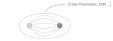
\includegraphics[scale=0.7]{motiflevel_ex.pdf}

\medskip

This geometrical information can be encoded quantitatively with continuous symmetry measures, local structure order parameters, etc., depending on task


\end{frame}


\begin{frame}{Extending Message Passing to Hypergraphs}

Now, we need a suitable convolutional structure that applies to hypergraphs...

\medskip

In this case, the neighborhood of nodes relevant to each message are now a set (instead of the single neighboring node feature of classic MPNNs)

\begin{gather*}
m_i^{t+1}=\sum_{h_j\ni x_i} M_t(n_i^{t},\underbrace{h_j^{t},\lbrace  n_w^t \vert n_w \in h_j }_{e_{ij},n_j}\rbrace)\\
\\
n_i^{t+1}=U_t(n_i^t,m_i^{t+1})\\
\end{gather*}
\end{frame}



\begin{frame}{Hypergraph Convolution}
To deal with the variable sized neighborhoods of features, we simply aggregate the neighborhood features in the message passing phase, so that we essentially have the following form of convolution:
\begin{align*}
x_i \rightarrow x_i &+ f_b(x_i\oplus e_{ij} \oplus \text{AGG}(\lbrace x_i, x_j\rbrace))\\
&+ f_m(x_i\oplus m_{j} \oplus \text{AGG}(\lbrace  n_w^t \vert n_w \in m_j \rbrace))
\end{align*}
where we only consider pair-wise and local environment hyperedges above (with other order structures, such as triplet and unit cell level hyperedges also fitting into this framework)

\end{frame}

\begin{frame}{Preliminary Results}
Preliminary test results suggest this local environment feature benefits most predicitive tasks!

\vspace{0.8cm}

Let's compare performance for crystal graphs, with only bond-level edges, to crystal hypergraphs with bond and local-environment hyperedges (using the same convolutional strucuture for both) on the Materials Project dataset.
\end{frame}


\begin{frame}{Preliminary Results: Band Gap}
\includegraphics[scale=0.3]{bvsbm.png}

Here, purple is for bond-only graphs; while grey is for bond and motif level hypergraphs.
\end{frame}



\begin{frame}{Preliminary Results: Formation Energy}
\includegraphics[scale=0.3]{bvsbm_form.png}

Here, green is for bond-only graphs; while blue is for bond and motif level hypergraphs.
\end{frame}




\end{document}